% =============================================================================
% FILE NAME : results_and_discussion.tex
% DEPARTMENT: University of Tuebingen
% AUTOR     : Tom Schammo
% =============================================================================
% CONTENT   : Include for chapter "Results and Discussion"
% =============================================================================


\section{Microphones}

\subsection{Implementation}

Driver support for $I^2S$ and PDM has already been implemented into the PULPissimo HAL \cite[Cha 4.3.7]{rust_pulp}.
Unfortunately, however, the microphones did not work right away for reasons listed below.
Unlike the PDM microphone, the $I^2S$ microphone does not work on the PULPissimo chip, due to a hardware compatibility issue.
The $I^2S$ microphone sends a total of 24 bits, one 18-bit word, and 6 zero bits, but the PULPissimo can only handle 16 bits.
While the PDM microphone is compatible with the PULPissimo chip, the Rust drivers were not mature enough for it to work using Rust.
Aside from the occasional small bug, the driver was missing some crucial features, due to a lack of documentation.
The PULPissimo data sheet \cite[Cha 4.8.67]{pulpissimo_datasheet} is missing two fields in the \emph{\lstinline{I2S_PDM_SETUP}} register.
Namely, \emph{\lstinline{PDM_ENABLE}} and \emph{\lstinline{PDM_MODE}}, which had to be implemented to enable PDM.
After these had been implemented PDM could be enabled.

\subsection{Experiments}

To test the functionality of the microphones I played a \SI{1}{\kilo\hertz} sine wave\footnote{Sine wave audio: \url{https://www.youtube.com/watch?v=3FBijeNg_Gs}},
which I then recorded using the microphone.

\subsubsection{I2S Microphone}

\begin{figure}[H]
    \centering
    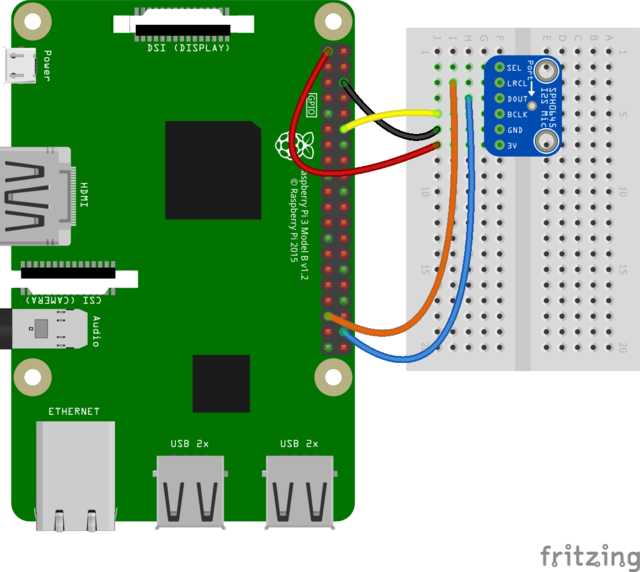
\includegraphics[width=0.5\textwidth]{figures/i2s/wiring_pi.png}
    \caption[$I^2S$ microphone wiring diagram with Raspberry Pi \cite{i2s_wiring}]{$I^2S$ microphone wiring diagram with Raspberry Pi}
    \label{fig:i2s_wiring}
\end{figure}

The $I^2S$ microphone has been wired as displayed in Figure~\ref{fig:i2s_wiring} \cite{i2s_wiring}.
Additionally, SEL has been tied to ground.
The recording was made using the command in Listing~\ref{code:record},
where \emph{<file name>} is the name of the output file.

\begin{minipage}{\textwidth}
\begin{lstlisting}[style=colorEX,language=bash,caption={Recording Command},label={code:record}]
arecord -D dmic_sv -c2 -r 48000 -f S32_LE -t wav -V mono -v <file name>
\end{lstlisting}
\end{minipage}

This creates a 32-bit, PCM-encoded mono WAVE audio file with a sample rate of \SI{48000}{\hertz}.
The \SI{1}{\kilo\hertz} sine wave audio has been played using the speakers of a Redmi Note 7 phone.

\begin{figure}[H]
    \centering
    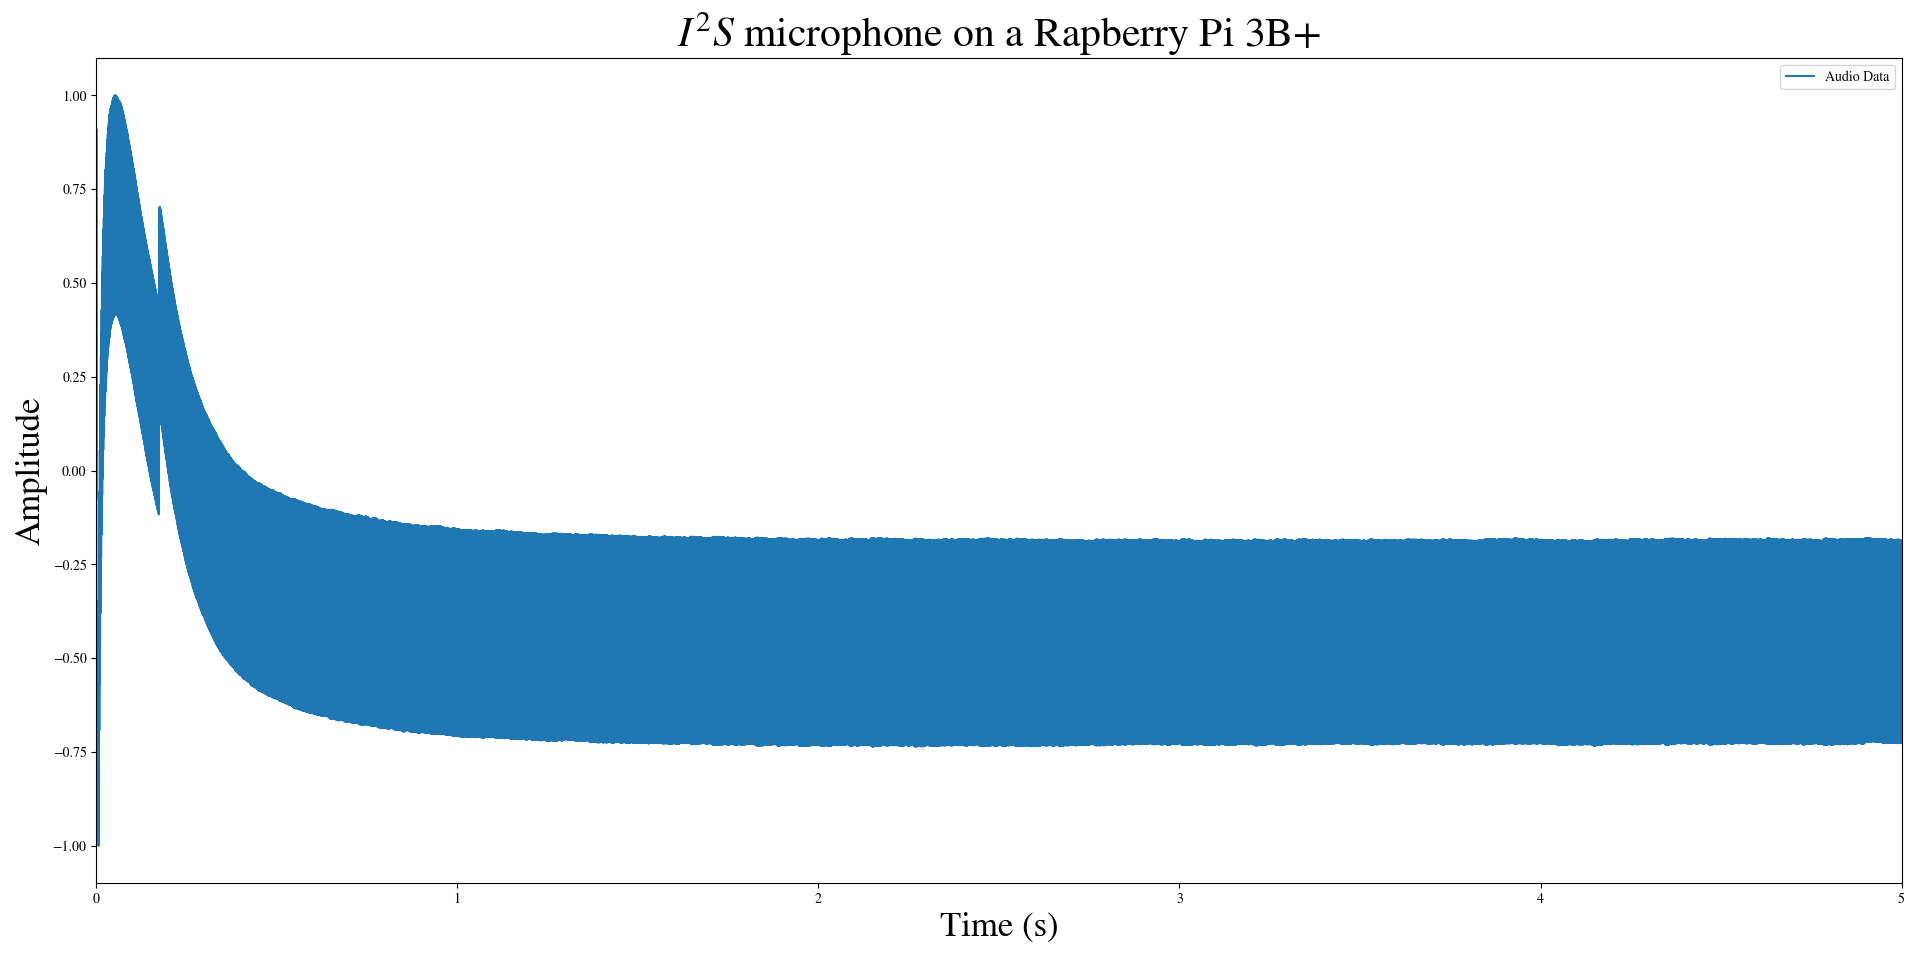
\includegraphics[width=0.9\textwidth]{figures/i2s/i2s_raw_data.png}
    \caption[PCM data of the $I^2S$ microphone normalized and plotted]{PCM data of the $I^2S$ microphone normalized plotted}
    \label{fig:i2s_raw}
\end{figure}

When analyzing the 5-second audio data capture displayed in Figure~\ref{fig:i2s_raw}, the spike from seconds 0 to about 0.5
is very noticeable. That is because the microphone seems to have a 'warm-up time', it takes about 1 second for it to be operational and produce clean data.
This has also been noticed on the PULPissimo board with the PDM microphone.
However, after that period, the $I^2S$ microphone is completely operational.
When zooming in and looking closer, the signal reveals a clean \SI{1}{\kilo\hertz} sine wave, as shown in Figure~\ref{fig:i2s_section}.

\begin{figure}[H]
    \centering
    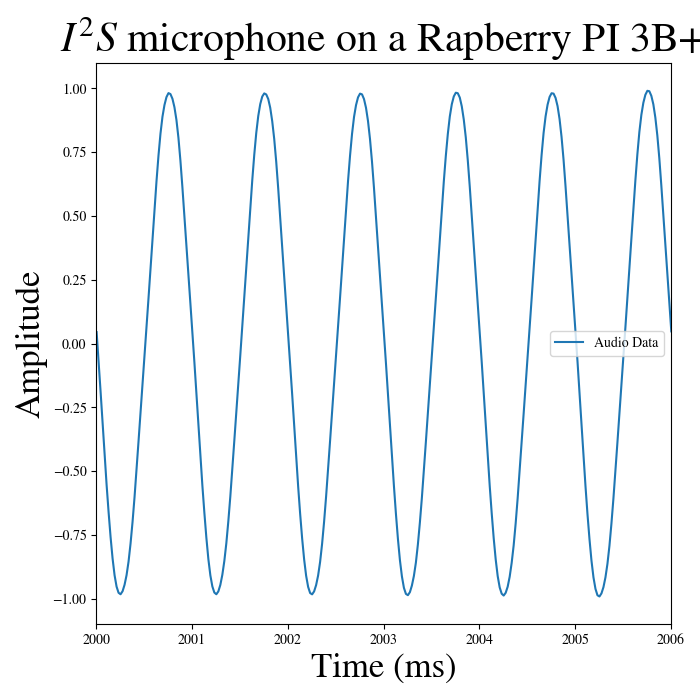
\includegraphics[width=0.9\textwidth]{figures/i2s/i2s_data_recording.png}
    \caption[Sample of normalized PCM data from $I^2S$ microphone]{Sample of normalized PCM data from $I^2S$ microphone}
    \label{fig:i2s_section}
\end{figure}

When taking a close look at a single period and overlaying the data with a perfect sine wave of the same
frequency, displayed in Figure~\ref{fig:i2s_period}, there is a slight, but noticeable discrepancy between the perfect sine
wave and the audio data.
This could have a variety of reasons.
Firstly, the audio that has been played might not have been a perfect sine wave to begin with.
There could've also been variations due to the speakers that had been used, the speakers
might not have produced a 100\% accurate tone.
Or this discrepancy could also be caused by something on the recording side.
Perhaps it is a result of microphone limitations.

\begin{figure}[H]
    \centering
    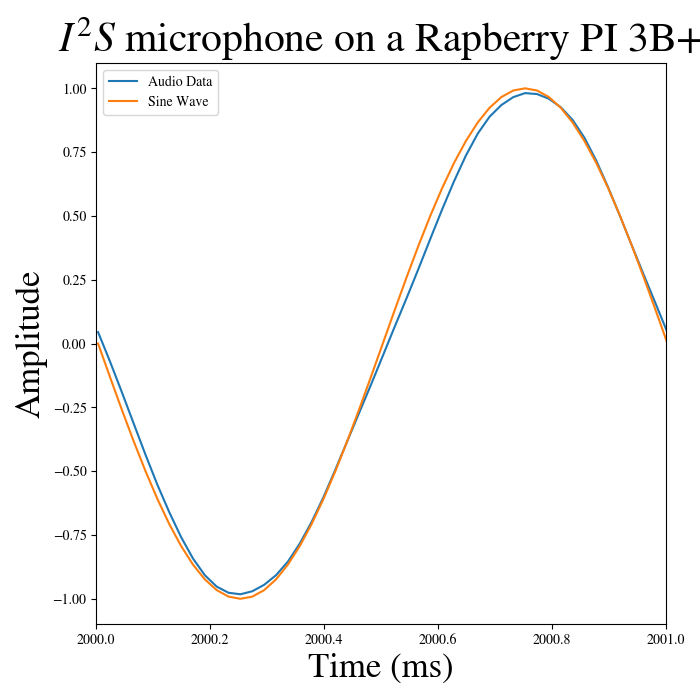
\includegraphics[width=0.9\textwidth]{figures/i2s/i2s_one_period.png}
    \caption[A single period of the normalized audio data, overlaid with a perfect 1kHz sine wave]{Single period of the normalized audio data, overlaid with a 1kHz sine wave}
    \label{fig:i2s_period}
\end{figure}

\subsubsection{PDM Microphone}

Several setups have been tested with the PDM microphone.
Probably the simplest setup would be to connect CLK, DAT, SEL, GND, and 3V (also sometimes referred to as $V_{DD}$) on the microphone
to \lstinline{I2S0_SCK} (clock of the $I^2S$ bus), \lstinline{I2S0_SDI} (data line of the $I^2S$ bus), \lstinline{I2S0_WS} (word select), GND (ground),
and \lstinline{+3V VOUT} (\SI{3.3}{\volt} output) on the development board respectively,
which are all listed in the development board reference manual \cite{pulpissimo}.
However, I decided to tie SEL to ground, since there was no intention of using stereo audio in the first place.\\
Furthermore, the decision to use a logic level converter\footnote{\url{https://cdn-shop.adafruit.com/datasheets/txb0108.pdf}}
has been made to protect the board and avoid potential problems due to voltage differences between the data and clock lines.
The PULPissimo runs internally on \SI{1.8}{\volt}, which is also the voltage level of the $I^2S$ clock pin.
However, according to the data sheet, the PDM microphone requires \SI{3.3}{\volt}.
So one end of the logic level converter is set to \SI{1.8}{\volt}, which is the side that the development board
is connected to, while the other end is set to \SI{3.3}{\volt}, which is the side that the microphone is connected to.
So the microphone receives \SI{3.3}{\volt} for the clock signal and the power source, and has an output voltage level
of \SI{3.3}{\volt} on the data line,
while the board has an output of \SI{1.8}{\volt} on its clock line and the data it receives from the microphone is also
converted to \SI{1.8}{\volt}.
The final wiring of the PDM microphone is shown in Figure~\ref{fig:pdm_wiring}.

\begin{figure}[H]
    \centering
    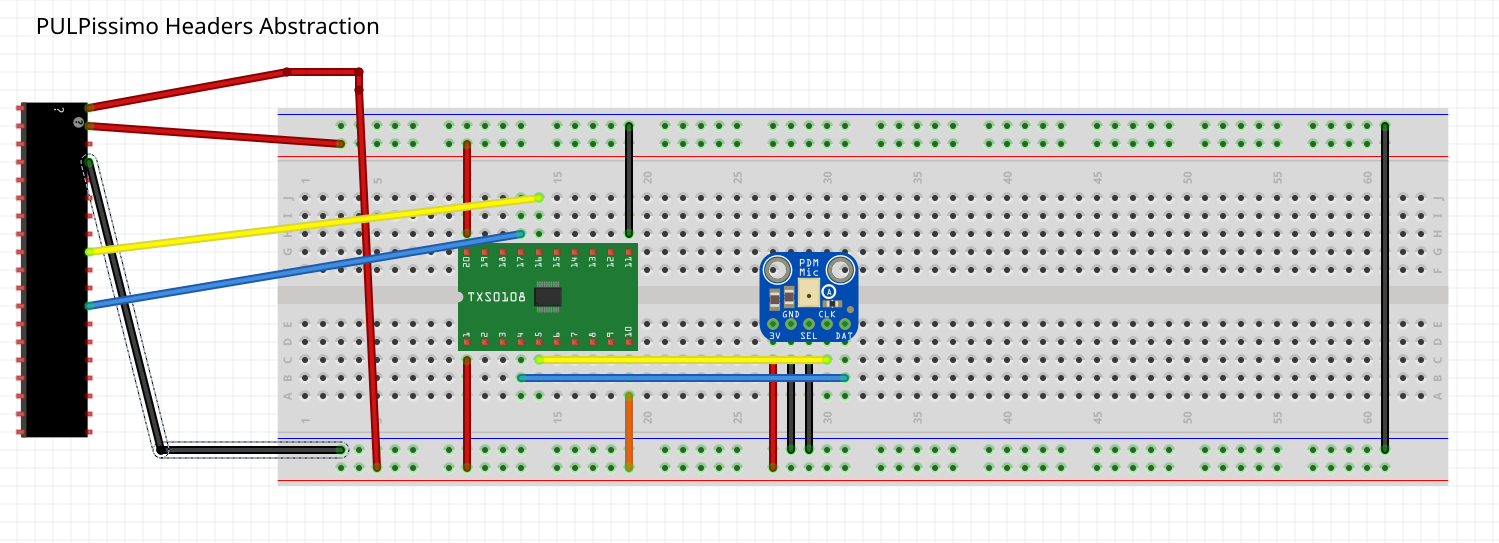
\includegraphics[width=0.9\textwidth]{figures/pdm/wiring.png}
    \caption[PDM microphone wiring with an abstraction for the PULPissimo]{PDM microphone wiring}
    \label{fig:pdm_wiring}
\end{figure}

As shown in the Listing~\ref{code:pdm_config}, the peripheral frequency on the board is set to \SI{212.5}{\mega\hertz}
and the sampling rate of the PDM microphone is set to \SI{16}{\kilo\hertz} with a decimation factor of 7.
This results in about a \SI{1}{\mega\hertz} clock frequency on the $I^2S$ bus, as shown in Figure~\ref{fig:i2s_capture}.
However, this is not exactly 'PDM data', since the driver did not enable PDM for the reasons discussed in the 'Implementation' section.

\begin{minipage}{\textwidth}
\begin{lstlisting}[style=colorEX,language=Rust,caption={Configuration of the board clock and the PDM driver},label={code:pdm_config}]
let clock = Clock::from_external(20_000_000u32.Hz(), 212_500_000u32.Hz());

let conf = i2s::Config {
    frequency: 16000,
    decimation_log2: 7,
    pdm: true,
    dual: false,
};
\end{lstlisting}
\end{minipage}

\begin{figure}[H]
    \begin{center}
        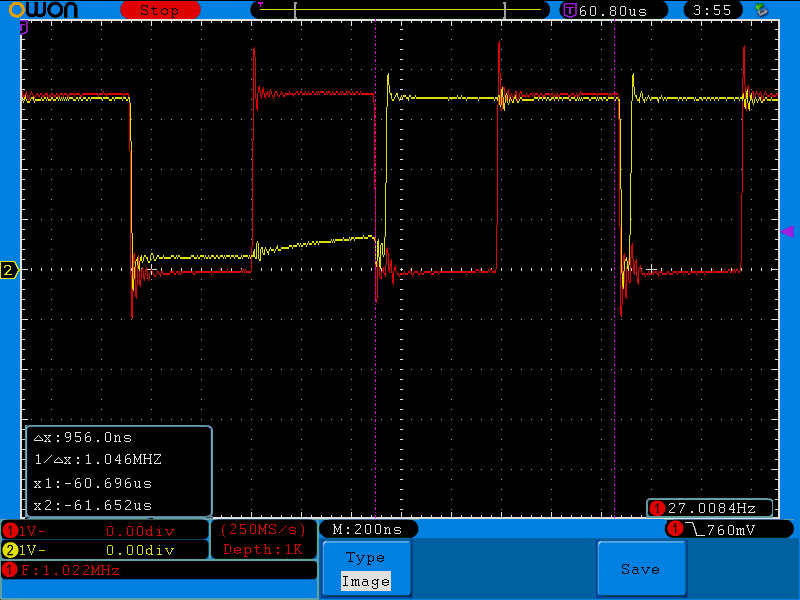
\includegraphics[width=0.5\textwidth]{figures/i2s_capture.png}
    \end{center}
    \caption[Oscilloscope capture of the microphone's data line (yellow) and clock line (red)]{Oscilloscope capture of the microphone's data line (yellow) and clock line (red)}
    \label{fig:i2s_capture}
\end{figure}

\begin{figure}[H]
    \begin{center}
        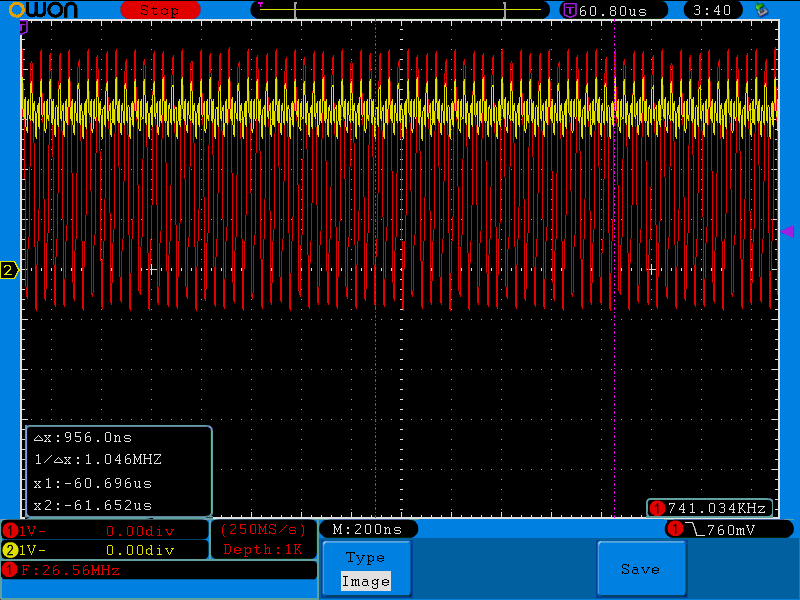
\includegraphics[width=0.5\textwidth]{figures/pdm_broken.png}
    \end{center}
    \caption[Oscilloscope capture of a PDM recording with PDM enabled]{Oscilloscope capture of a PDM recording with PDM enabled}
    \label{fig:pdm_no_config}
\end{figure}

After modifying the driver code to support PDM as described in the 'Implementation' section of this chapter,
the program no longer outputs any data (only 0-byte values), and the oscilloscope output is shown in Figure~\ref{fig:pdm_no_config}.
It is immediately obvious that something is wrong.
The reason for this behavior is that the board's PDM clock was disabled after causing problems because PDM was not enabled to begin with.
After re-enabling the PDM clock the signal looks as depicted in Figure~\ref{fig:pdm_working}.
This changes the frequency of the $I^2S$ clock, so after adjusting the configuration the microphone is ready for testing.

\begin{figure}[H]
    \begin{center}
        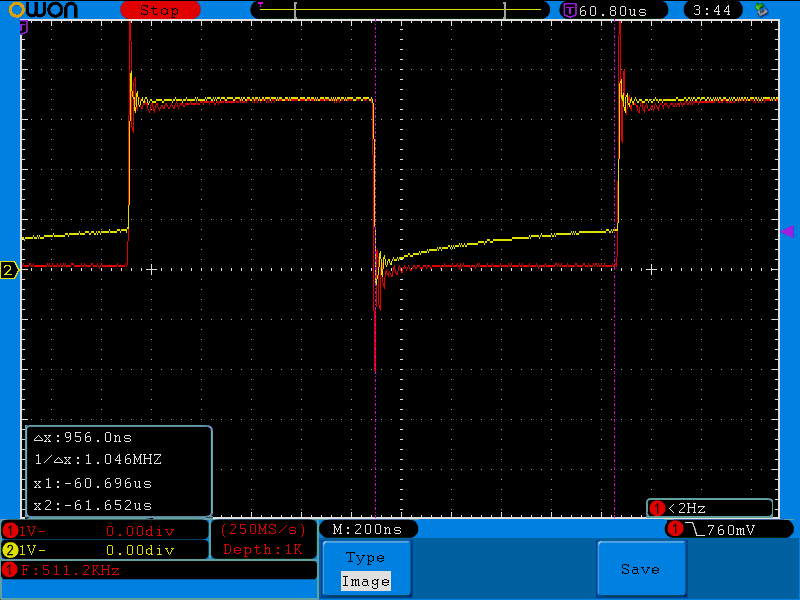
\includegraphics[width=0.5\textwidth]{figures/pdm_working.png}
    \end{center}
    \caption[Oscilloscope capture of the PDM microphone's data line (yellow) and clock line (red) after everything is enabled]
    {Oscilloscope capture of the PDM microphone's data line (yellow) and clock line (red) after everything is enabled}
    \label{fig:pdm_working}
\end{figure}

\begin{minipage}{\textwidth}
The microphone has been tested with two different configurations displayed in Listing~\ref{code:pdm_config_ready} and Listing~\ref{code:pdm_config_high}.
Both have the decimation factor increased to 8, and one uses a sampling rate of \SI{16}{\kilo\hertz} while the other uses a sampling rate of \SI{48}{\kilo\hertz}.

\begin{lstlisting}[style=colorEX,language=Rust,caption={Updated configuration of the PDM microphone with a 16kHz sampling rate},label={code:pdm_config_ready}]
let conf = i2s::Config {
    frequency: 16000,
    decimation_log2: 8,
    pdm: true,
    dual: false,
};
\end{lstlisting}

\begin{lstlisting}[style=colorEX,language=Rust,caption={Updated configuration of the PDM microphone with a 48kHz sampling rate},label={code:pdm_config_high}]
let conf = i2s::Config {
    frequency: 48000,
    decimation_log2: 8,
    pdm: true,
    dual: false,
};
\end{lstlisting}
\end{minipage}

\begin{figure}[H]
    \begin{center}
        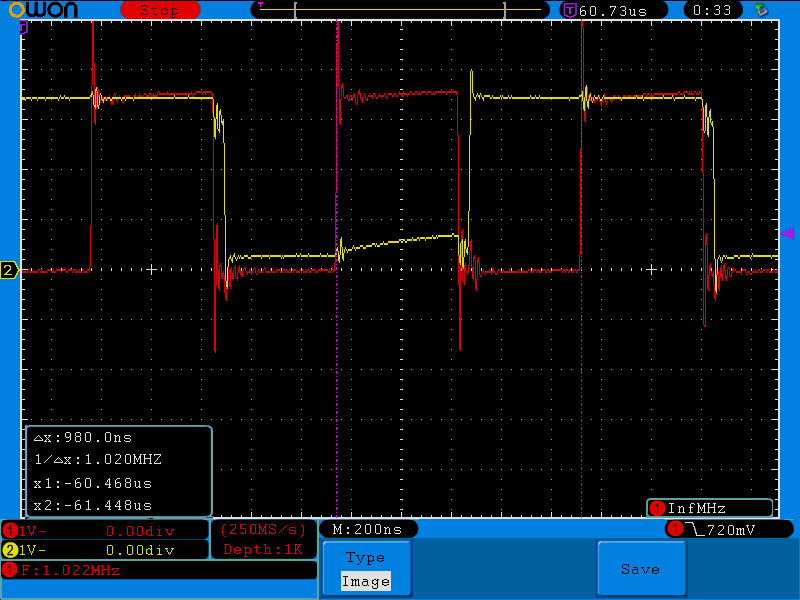
\includegraphics[width=0.5\textwidth]{figures/16k_1mhz_sine.png}
    \end{center}
    \caption[Oscilloscope capture of the PDM microphone's data line (yellow) and clock line (red) at a 16kHz sampling rate]
    {Oscilloscope capture of the PDM microphone's data line (yellow) and clock line (red) at a 16kHz sampling rate}
    \label{fig:pdm_16k}
\end{figure}

A sampling rate of \SI{16}{\kilo\hertz} and \SI{48}{\kilo\hertz} with a decimation factor of 8
result in a clock frequency of approximately \SI{1}{\mega\hertz} and \SI{3}{\mega\hertz} respectively,
which is one at the low and one at the high end of the clock frequency range at which the PDM
microphone operates at.
The corresponding oscilloscope captures are shown in Figure~\ref{fig:pdm_16k} and Figure~\ref{fig:pdm_48k}.

\begin{figure}[H]
    \begin{center}
        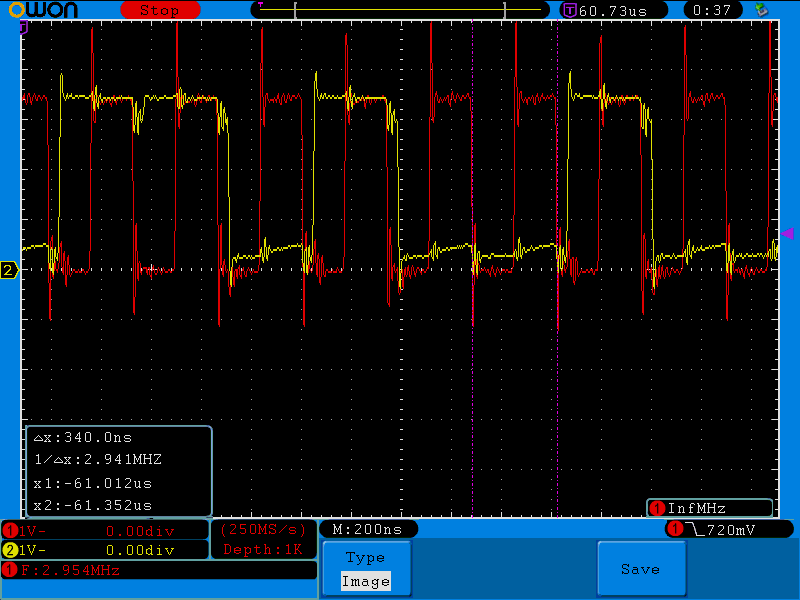
\includegraphics[width=0.5\textwidth]{figures/48k_3mhz_sine.png}
    \end{center}
    \caption[Oscilloscope capture of the PDM microphone's data line (yellow) and clock line (red) at a 48kHz sampling rate]{Oscilloscope capture of the PDM microphone's data line (yellow) and clock line (red) at a 48kHz sampling rate}
    \label{fig:pdm_48k}
\end{figure}

When analyzing the PCM data from these captures it is clear that the driver is not working as intended.
Figure~\ref{fig:pdm_rust_16k} shows the signal with a sampling rate of \SI{16}{\kilo\hertz} and
Figure~\ref{fig:pdm_rust_48k} shows the signal with a sampling rate of \SI{48}{\kilo\hertz}.

\begin{figure}[H]
    \centering
    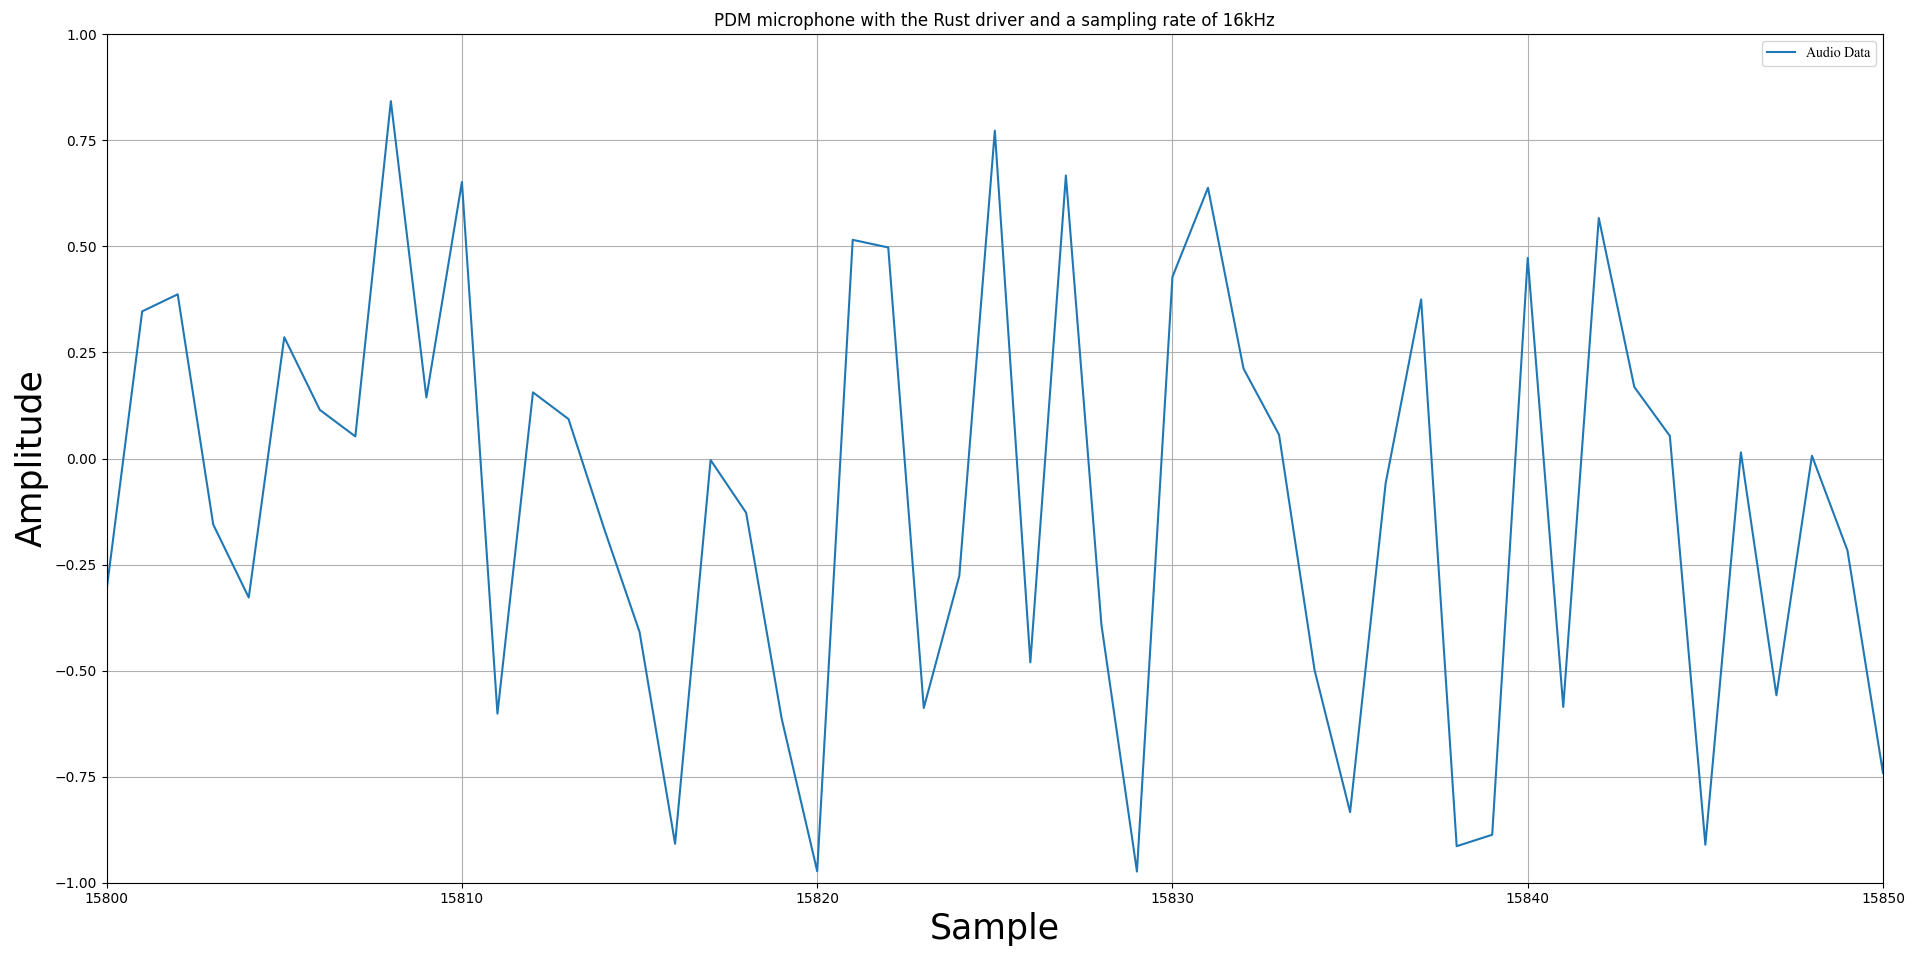
\includegraphics[width=0.9\textwidth]{figures/pdm/pdm_rust_16k.png}
    \caption[Segment of the normalized audio data recorded by the PDM microphone using the Rust driver with a sampling rate of 16kHz]
    {Segment of the normalized audio data recorded by the PDM microphone using the Rust driver with a sampling rate of 16kHz}
    \label{fig:pdm_rust_16k}
\end{figure}

\begin{figure}[H]
    \centering
    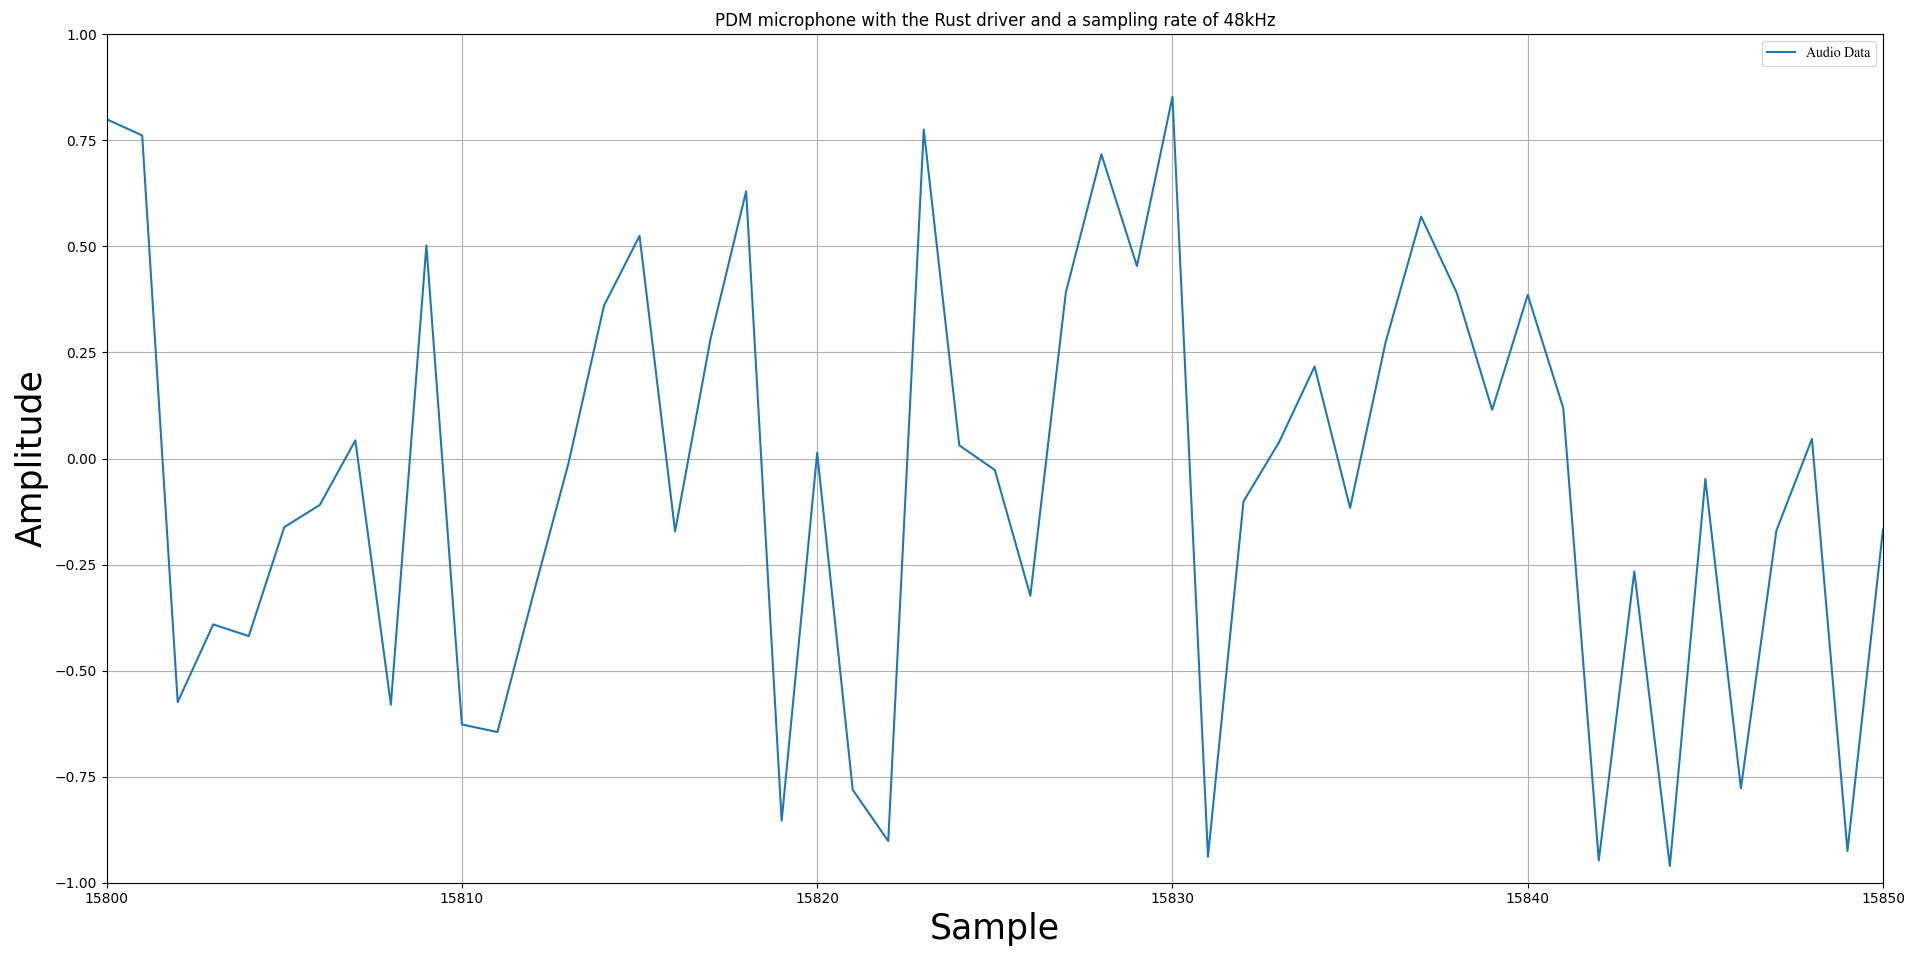
\includegraphics[width=0.9\textwidth]{figures/pdm/pdm_rust_48k.png}
    \caption[Segment of the normalized audio data recorded by the PDM microphone using the Rust driver with a sampling rate of 48kHz]
    {Segment of the normalized audio data recorded by the PDM microphone using the Rust driver with a sampling rate of 48kHz}
    \label{fig:pdm_rust_48k}
\end{figure}

Neither displays anything resembling a sine wave.
What is expected is something that looks like Figure~\ref{fig:pdm_c}, which was recorded with the same microphone and wiring using the C driver.
It is not clear what caused the recording to be inaccurate.
Presumably, there still is at least one bug in the driver.
The oscillations shown in Figures~\ref{fig:pdm_16k} and \ref{fig:pdm_48k} also seem very suspicious.
They are especially dominant on the clock signal, but they are also present on the data signal.

\begin{figure}[H]
    \centering
    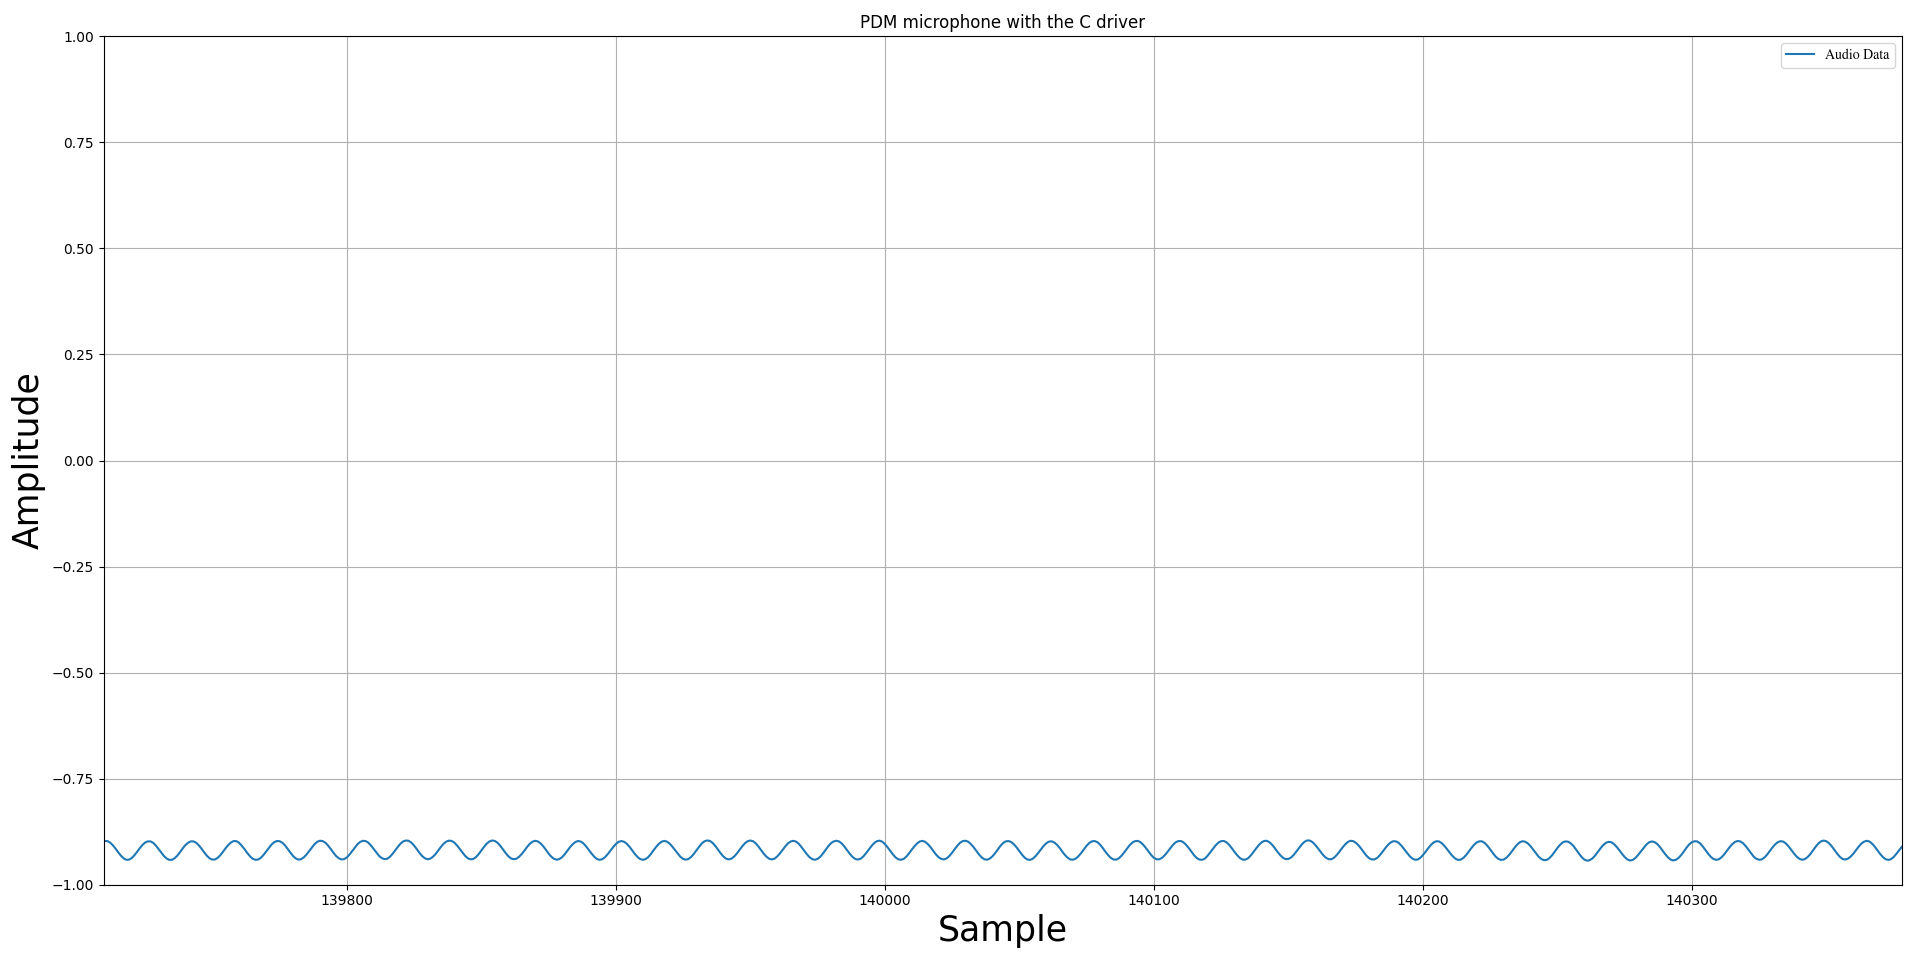
\includegraphics[width=0.9\textwidth]{figures/pdm/pdm_c.png}
    \caption[Segment of the normalized audio data recorded by the PDM microphone using the C driver]{Segment of the normalized audio data recorded by the PDM microphone using the C driver}
    \label{fig:pdm_c}
\end{figure}

\begin{minipage}{\textwidth}
\section{UltraTrail}

\subsection{Implementation}

To implement the driver for UltraTrail, it first has to be added to the SVD file in the PAC
as a peripheral to generate the necessary Rust code to access hardware registers.
Subsequently, the driver can be implemented in the HAL crate.
Finally, I have ported a small program from C to Rust, that contains a set of pre-defined
weights, bias and feature inputs, as well as expected results.
This program can be used to test the implementation of the driver, as it also
performs different configurations by reading and writing the different registers.
\\\\
However, there have been a few differences when it comes to the implementation details.
Most importantly, the C drivers for the PULPissimo provide the \lstinline{__rt_periph_wait_event} function,
which is a sophisticated busy wait.
The test code uses that function to wait for UltraTrail to trigger an event interrupt, to announce that
it is done processing as shown in Listing~\ref{code:c_wait_for_event}.
\end{minipage}

\begin{minipage}{\textwidth}
\begin{lstlisting}[style=colorEX,language=C,caption={Waiting for the event in C},label={code:c_wait_for_event}]
pacc_start();

soc_eu_fcEventMask_setEvent(ARCHI_SOC_EVENT_FCHWPE0);
__rt_periph_wait_event(ARCHI_SOC_EVENT_FCHWPE0, 1);

pacc_stop();
\end{lstlisting}
\end{minipage}

However, that function has not been implemented in the Rust drivers, so I had to slightly
vary the implementation of the test code.\\
First I had to define a Mutex \footnote{\url{https://doc.rust-lang.org/std/sync/struct.Mutex.html}}
for the event state, to monitor whether an event interrupt has been triggered as demonstrated
in Listing~\ref{code:mutex}.

\begin{lstlisting}[style=colorEX,language=Rust,caption={Definition of the necessary Mutexes},label={code:mutex}]
static EVENT_STATE: Mutex<Cell<bool>> = Mutex::new(Cell::new(false));
\end{lstlisting}

Subsequently, I defined an event handler as presented in Listing~\ref{code:event_handler}, which
stops the accelerator when it is done and changes the global event state Mutex.

\begin{minipage}{\textwidth}
\begin{lstlisting}[style=colorEX,language=Rust,caption={Event handler function},label={code:event_handler}]
fn hwpe_event_handler() {
    interrupt::free(|cs| {
        unsafe {
            Accelerator::stop_steal();
        }

        EVENT_STATE.borrow(*cs).set(true);
    })
}
\end{lstlisting}
\end{minipage}

After that I just had to enable the event and set the event handler to deal with the event when it is triggered.
The code of that can be seen in Listing~\ref{code:enable_event}.

\begin{minipage}{\textwidth}
\begin{lstlisting}[style=colorEX,language=Rust,caption={Code to enable the hardware event and set the handler},label={code:enable_event}]
unsafe {
    event_interrupt.enable_event(EventId::Hwpe0);
    event_interrupt.set_event_handler(EventId::Hwpe0, hwpe_event_handler);
}
\end{lstlisting}
\end{minipage}

Finally, I could write the busy wait, which does nothing until the interrupt is received
and then changes the event state.
An example of that is displayed in Listing~\ref{code:busy_wait}

\begin{minipage}{\textwidth}
\begin{lstlisting}[style=colorEX,language=Rust,caption={Snippet of the busy wait that waits for UltraTrail to finish},label={code:busy_wait}]
accelerator.start();

let mut event = false;
while !event {
    wait_x_nops(1000);

    interrupt::free(|cs| {
        if EVENT_STATE.borrow(*cs).get() {
            event = true;
            EVENT_STATE.borrow(*cs).set(false);
        }
    })
}

// ...
\end{lstlisting}
\end{minipage}

\subsection{Experiments}

The expected results are stored in a vector containing 12 16bit integers, displayed in the Listing~\ref{code:acc_results}.

\begin{minipage}{\textwidth}
\begin{lstlisting}[style=colorEX,language=Rust,caption={The expected results from the driver test},label={code:acc_results}]
let correct_results = [
    0xf246, 0x16bf, 0x08a0, 0xfe52, 0xf709, 0xef58, 0xff6b, 0xf946, 0xfebd, 0x0f40, 0xee45, 0x18f0,
];
\end{lstlisting}
\end{minipage}

When comparing the code in Listing~\ref{code:acc_results} to the minicom output shown in \ref{code:minicom_out_acc},
one realizes that they match. Which leads me to believe that the UltraTrail driver works as intended.

\begin{minipage}{\textwidth}
\begin{lstlisting}[style=colorEx,caption={Minicom output after executing the driver test},label={code:minicom_out_acc}]
result #0: 0xf246
result #1: 0x16bf
result #2: 0x8a0
result #3: 0xfe52
result #4: 0xf709
result #5: 0xef58
result #6: 0xff6b
result #7: 0xf946
result #8: 0xfebd
result #9: 0xf40
result #10: 0xee45
result #11: 0x18f0
\end{lstlisting}
\end{minipage}
